\subsection{Homotopy Groups}\label{ssec:structure-group}

In this section we define algebraic invariants of cubesets: their structure groups,
also known as homotopy groups in analogy to simplicial sets.

\begin{definition}\label{def:structure-group}
Let $X$ be an $n$-step cubeset, $x_0\in X(0)$ a point and $n\geq 1$.
Then define $\pi_n(X,x_0)$ to be the set
\[
    \{ c\colon{\bbox}^n\to X \mid c\lvert_{{\bbcor}^n} \equiv x_0 \}.
\]
We define a binary operation on $\pi_n(X,x_0)$ as follows.
Let $a,b\in\pi_n(X,x_0)$ and set $\lambda_i\colon{\bbox}^n\to X$ to be $\lambda_1 = a$, $\lambda_2 = b$ and $\lambda_i \equiv x_0$ for $2<i\le n+1$.
This defines a corner $\lambda_{a,b}\colon{\bbcor}^{n+1}\to X$ which admits a unique completion $\overline{a*b}\colon{\bbox}^{n+1}\to X$ to a cube in $X$.
Let $s\colon{\bbox}^n\to{\bbox}^{n+1}$ be the diagonal $(x_1,\ldots,x_n)\mapsto (x_1,x_1,x_2,\ldots,x_n)$.
Then define
\[
    a * b = \overline{a*b}\circ s \colon {\bbox}^n\to X.
\]
With this operation, we call $\pi_n(X,x_0)$ the \emph{$n$-th structure monoid of $X$.}
\end{definition}


Let us illustrate this definition in the cases $n=1$ and $n=2$
where the resulting composition $a*b$ is colored red.
\begin{center}
\begin{tikzcd}[column sep=small, row sep= small]
	&&&&& b && {a*b} \\
	b && {a*b} && {x_0} && a \\
	&&&&& {x_0} && {x_0} \\
	{x_0} && a && {x_0} && {x_0}
	\arrow[no head, from=1-6, to=1-8]
	\arrow[dashed, no head, from=1-6, to=3-6]
	\arrow[no head, from=2-1, to=2-3]
	\arrow[no head, from=2-5, to=1-6]
	\arrow[color={rgb,255:red,214;green,92;blue,92}, no head, from=2-5, to=1-8]
	\arrow[no head, from=2-5, to=2-7]
	\arrow[color={rgb,255:red,214;green,92;blue,92}, no head, from=2-5, to=4-5]
	\arrow[no head, from=2-7, to=1-8]
	\arrow[dashed, no head, from=3-6, to=3-8]
	\arrow[color={rgb,255:red,214;green,92;blue,92}, no head, from=3-8, to=1-8]
	\arrow[no head, from=4-1, to=2-1]
	\arrow[color={rgb,255:red,214;green,92;blue,92}, no head, from=4-1, to=2-3]
	\arrow[no head, from=4-1, to=4-3]
	\arrow[no head, from=4-3, to=2-3]
	\arrow[dashed, no head, from=4-5, to=3-6]
	\arrow[color={rgb,255:red,214;green,92;blue,92}, dashed, no head, from=4-5, to=3-8]
	\arrow[no head, from=4-5, to=4-7]
	\arrow[no head, from=4-7, to=2-7]
	\arrow[no head, from=4-7, to=3-8]
\end{tikzcd}
\end{center}


\begin{remark}
A priori, the choice of $s$ for extracting an $n$-cube out of the completed ($n+1$)-cube
seems arbitrary.
However, it essentially is the only choice:
given two inerts $\epsilon_i,\epsilon_j\colon{\bbox}^n\to{\bbox}^{n+1}$ with $i\neq j$,
there is exactly one subobject of ${\bbox}^{n+1}$ that is the complement of the symmetric difference of $\epsilon_i$ and $\epsilon_j$.
This is due to the fact that the complement of the symmetric difference of $\epsilon_i$ and $\epsilon_j$
is equal to the subobject $[\omega_i=\omega_j=0]\cup[\omega_i=\omega_j=1]$ of dimension $n$,
since it consists of $2\cdot 2^{n-1} = 2^n$ points.
We also see that it doesn't matter in the definition of the operation that we impose $a$ and $b$
on the sides $\epsilon_1$ and $\epsilon_2$, it could have also been any other two distinct lower faces.%
\footnote{In fact, since flips and coordinate permutations induce automorphisms on the set of $n+1$-cubes, making the same definition after some automorphism of $\bbox^{n+1}$ leads to the same composition on concrete cubesets.}
\end{remark}

The next proposition justifies the definition of structure \emph{monoid}.

\begin{proposition}\label{prop:structure-group-is-monoid}
The operation
\[
    *\colon\pi_n(X,x_0)\times\pi_n(X,x_0)\to\pi_n(X,x_0),\quad (a,b)\mapsto a*b
\]
makes $\pi_n(X,x_0)$ an abelian monoid.
This construction upgrades to a functor $\cSet_{\ast,n}\to\cMon$.
\end{proposition}

\begin{proof}
\textbf{Commutativity:}
Let $a,b\in\pi_n(X,x_0)$.
In order to show that $a*b = b*a$ we want to see that
one can act on the ($n+1$)-cube witnessing the composition by an automorphism that interchanges $a$ with $b$ but leaves the rest of the cube, and in particular the side inducing the composition, invariant.
This can be described for $n=1$ by the following diagram
\begin{center}
\begin{tikzcd}
	b & {a*b} & a & {b*a} \\
	{x_0} & a & {x_0} & b
	\arrow[no head, from=1-1, to=1-2]
	\arrow[no head, from=1-3, to=1-4]
	\arrow[no head, from=2-1, to=1-1]
	\arrow[color={rgb,255:red,214;green,92;blue,92}, no head, from=2-1, to=1-2]
	\arrow[no head, from=2-1, to=2-2]
	\arrow[""{name=0, anchor=center, inner sep=0}, no head, from=2-2, to=1-2]
	\arrow[""{name=1, anchor=center, inner sep=0}, no head, from=2-3, to=1-3]
	\arrow[color={rgb,255:red,214;green,92;blue,92}, no head, from=2-3, to=1-4]
	\arrow[no head, from=2-3, to=2-4]
	\arrow[no head, from=2-4, to=1-4]
	\arrow["\leftrightsquigarrow"{description}, draw=none, from=0, to=1]
\end{tikzcd}
\end{center}
where the $2$-cubes relate by switching the coordinates $x_1$ and $x_2$.
This argument works in every dimension and is formalized as follows.

For $k\geq 2$ denote by $\sigma_{12}^k\in\Aut({\bbox}^{k})$ the automorphism exchanging coordinates $x_1$ and $x_2$.
Note that $\sigma_{12}^k$ maps the corner onto the corner,
i.e., restricts to an automorphism $\sigma_{12}^k\rvert\colon{\bbcor}^k\to{\bbcor}^k$.
We first show that $\overline{b*a}\circ\sigma_{12}^{n+1} = \overline{a*b}$.
Since $X$ is $n$-step it suffices to see that $\lambda_{b,a}\circ\sigma_{12}^{n+1}\rvert = \lambda_{a,b}$.
But this can be tested against inerts $\epsilon_i\colon{\bbox}^n\to{\bbcor}^{n+1}$.
There we have that $\sigma_{12}^{n+1}\rvert\circ\epsilon_i = \epsilon_i\circ\sigma_{12}^n$ for $i\geq 3$
and $\sigma_{12}^{n+1}\rvert\circ\epsilon_1 = \epsilon_2$, $\sigma_{12}^{n+1}\rvert\circ\epsilon_2 = \epsilon_1$
since $\sigma_{12}^{n+1}$ can be decomposed as
\[
    \sigma_{12}^2\times\id\colon{\bbox}^2\times{\bbox}^{n-1}\to{\bbox}^2\times{\bbox}^{n-1}.
\]
This shows the desired equality for $i = 1,2$.
For $i\geq 3$ we have that
\[
      \lambda_{b,a}\circ\sigma_{12}^{n+1}\rvert\circ\epsilon_i
    = \lambda_{b,a}\circ\epsilon_i\circ\sigma_{12}^n
    = x_0\circ\sigma_{12}^n
    = x_0
    = \lambda_{a,b}\circ\epsilon_i,
\]
verifying the claim there as well.
From $\sigma_{12}^{n+1}\circ s = s$ we conclude that
\[
    a*b = \overline{a*b}\circ s = \overline{b*a}\circ\sigma_{12}^{n+1}\circ s = b*a.
\]

\textbf{Identity element:}
Clearly, the constant $n$-cube $x_0$ is the obvious candidate to be the neutral element.
To see that it actually is, consider the case $n=1$:
the $2$-cube
\begin{center}
\begin{tikzcd}
	{x_0} & a \\
	{x_0} & a
	\arrow[no head, from=1-1, to=1-2]
	\arrow[no head, from=2-1, to=1-1]
	\arrow[color={rgb,255:red,214;green,92;blue,92}, no head, from=2-1, to=1-2]
	\arrow[no head, from=2-1, to=2-2]
	\arrow[no head, from=2-2, to=1-2]
\end{tikzcd}
\end{center}
is a cube in $X$: it is the degeneration of $a$ into an additional dimension.
By definition of the operation, $a*x_0 = a$.

In general, let $d\colon{\bbox}^{n+1}\to{\bbox}^n$ denote the degeneracy omitting the first coordinate,
which is left inverse to both the inert $\epsilon_1$ and to the diagonal $s$.
Take $a\in\pi_n(X,x_0)$ and consider $a\circ d\colon{\bbox}^{n+1}\to X$.
Then $a\circ d\circ\epsilon_1 = a$.
For $i\geq 2$ we have that $d\circ\epsilon_i\colon{\bbox}^n\to{\bbox}^n$ factors through an inert face map, and hence $a\circ d\circ\epsilon_i \equiv x_0$.
Thus, $a\circ d = \overline{a*x_0}$ and
\[
    a*x_0 = \overline{a*x_0}\circ s = a\circ d\circ s = a.
\]
By commutativity, we also have $x_0*a = a$.
Thus, $x_0$ is the identity element of the monoid.

\textbf{Associativity:} Take elements $a,b,c\in\pi_n(X,x_0)$ and the ($n+1$)-cubes $\overline{a*b}$, etc.,
that witness their composition.
Together, they yield a corner of an ($n+2$)-cube.
We use unique corner completion in dimension $n+2$ to obtain a point $a*b*c$
witnessing $(a*b)*c$ and $a*(b*c)$ as $n$-dimensional subcubes,
so that they have to be the same.
The situation is summarized for $n=1$ by the following image,
where $\overline{(a*b)*c}$ is colored red, $\overline{a*(b*c)}$ blue and $(a*b)*c = a*(b*c)$ in yellow.
\begin{center}
\begin{tikzcd}[column sep=small, row sep=small]
	& {a*c} && a*b*c && {a*c} &&& a*b*c \\
	a && {a*b} && a &&& {a*b} \\
	& c && {b*c} && c &&& {b*c} \\
	{x_0} && b && {x_0} &&& b
	\arrow[dotted, no head, from=1-2, to=1-4]
	\arrow[no head, from=1-6, to=1-9]
	\arrow[no head, from=2-1, to=1-2]
	\arrow[no head, from=2-1, to=2-3]
	\arrow[no head, from=2-1, to=4-1]
	\arrow[dotted, no head, from=2-3, to=1-4]
	\arrow[no head, from=2-5, to=1-6]
	\arrow[color={rgb,255:red,92;green,92;blue,214}, no head, from=2-5, to=1-9]
	\arrow[no head, from=2-5, to=2-8]
	\arrow[color={rgb,255:red,214;green,92;blue,92}, no head, from=2-8, to=1-9]
	\arrow[dashed, no head, from=3-2, to=1-2]
	\arrow[dashed, no head, from=3-2, to=3-4]
	\arrow[dotted, no head, from=3-4, to=1-4]
	\arrow[dashed, no head, from=3-6, to=1-6]
	\arrow[color={rgb,255:red,214;green,92;blue,92}, dashed, no head, from=3-6, to=1-9]
	\arrow[dashed, no head, from=3-6, to=3-9]
	\arrow[color={rgb,255:red,92;green,92;blue,214}, no head, from=3-9, to=1-9]
	\arrow[dashed, no head, from=4-1, to=3-2]
	\arrow[no head, from=4-1, to=4-3]
	\arrow[no head, from=4-3, to=2-3]
	\arrow[no head, from=4-3, to=3-4]
	\arrow[color={rgb,255:red,214;green,214;blue,92}, dashed, no head, from=4-5, to=1-9]
	\arrow[color={rgb,255:red,92;green,92;blue,214}, no head, from=4-5, to=2-5]
	\arrow[color={rgb,255:red,214;green,92;blue,92}, no head, from=4-5, to=2-8]
	\arrow[color={rgb,255:red,214;green,92;blue,92}, dashed, no head, from=4-5, to=3-6]
	\arrow[color={rgb,255:red,92;green,92;blue,214}, dashed, no head, from=4-5, to=3-9]
	\arrow[no head, from=4-5, to=4-8]
	\arrow[no head, from=4-8, to=2-8]
	\arrow[no head, from=4-8, to=3-9]
\end{tikzcd}
\end{center}
Now to the formal argument:
denote $\lambda_1 = \overline{a*b}$, $\lambda_2 = \overline{a*c}$ and $\lambda_3 = \overline{b*c}$ the corresponding ($n+1$)-cubes
to the compositions $a*b$, $a*c$ and $b*c$, respectively (so that $\overline{a*b}\circ s = a*b$, etc.).
Let $\lambda_i \equiv x_0$ for $4\leq i\leq n+2$.
That these ($n+1$)-cubes $\lambda_i$ yield a corner $\lambda\colon{\bbcor}^{n+2}\to X$
can be verified by a direct computation using Remark~\ref{rem:corner-combinatorial}.
Now take the completion $d\colon{\bbox}^{n+2}\to X$ of $\lambda$.
We define the maps of cubes
\begin{align*}
    r\colon{\bbox}^{n+1}\to{\bbox}^{n+2},\quad &(x_1,\ldots,x_{n+1})\mapsto(x_1,x_2,x_2,x_3,\ldots,x_{n+1}) \\
    b\colon{\bbox}^{n+1}\to{\bbox}^{n+2},\quad &(x_1,\ldots,x_{n+1})\mapsto(x_1,x_1,x_2,\ldots,x_{n+1})
\end{align*}
which ought to extract $\overline{(a*b)*c}$ and $\overline{a*(b*c)}$, respectively, out of $d$.%
\footnote{As depicted in red ($r$) and blue ($b$) for $n=1$. If you can't see the colors, as, e.g., the second author, it doesn't matter, really.}
To see that $d\circ r = \overline{(a*b)*c}$ we need to verify that both cubes agree on their corner.
For $i=1$ we have that $r\circ\epsilon_1^n = \epsilon_1^{n+1}\circ s$,
so
\[
    d\circ r\circ\epsilon_1^n = d\circ\epsilon_1^{n+1}\circ s = \overline{a*b}\circ s = a*b.
\]
For $i=2$ we calculate $r\circ\epsilon_2^n = \epsilon_2^{n+1}\circ\epsilon_2^n$,
hence
\[
    d\circ r\circ\epsilon_2^n = d\circ\epsilon_2^{n+1}\circ\epsilon_2^n = \overline{a*c}\circ\epsilon_2^n = c.
\]
For $j\geq 3$ we obtain $r\circ\epsilon_j^n = \epsilon_{j+1}^{n+1}\circ r'$ for some (linear) $r'\colon{\bbox}^n\to{\bbox}^{n+1}$ and therefore,
\[
    d\circ r\circ\epsilon_j^n = d\circ\epsilon_{j+1}^{n+1}\circ r' = x_0\circ r' = x_0.
\]
This verifies the claim.
The analogous statement for $b$ is verified using similar arguments.
From the fact that $r\circ s = b\circ s$ we finally obtain
\[
    (a*b)*c = \overline{(a*b)*c}\circ s = d\circ r\circ s = d\circ b\circ s = a*(b*c)
\]
and so the operation is associative.

\textbf{Functoriality:}
If $f\colon(X,x_0)\to(Y,y_0)$ is a map of pointed $n$-step cubesets,
it preserves corners and the basepoint and so induces a map $f_\ast\colon\pi_n(X,x_0)\to\pi_n(Y,y_0)$.
Moreover, it is a monoid homomorphism since $f$ is a natural transformation and preserves corners.
\end{proof}

\begin{remark}\label{rem:structure-mon-not-grouplike}
In general, even for $n$-step $X$, the monoid $\pi_n(X,x_0)$ does in general not have inverses.
One would like to define, for $a\in\pi_n(X,x_0)$, an inverse $a^{-1}$ as follows (in case $n=1$):
we search for an element $a^{-1}\in\pi_1(X,x_0)$ such that the 2-cube on the left is in $X$,
and the red diagonal is the constant $x_0$.
\begin{center}
\begin{tikzcd}
	{a^{-1}} & {x_0} & {a^{-1}} & {x_0} \\
	{x_0} & a & {x_0} & a
	\arrow[no head, from=1-1, to=1-2]
	\arrow[dotted, no head, from=1-4, to=1-3]
	\arrow[no head, from=2-1, to=1-1]
	\arrow[color={rgb,255:red,214;green,92;blue,92}, no head, from=2-1, to=1-2]
	\arrow[no head, from=2-1, to=2-2]
	\arrow[no head, from=2-2, to=1-2]
	\arrow[dotted, no head, from=2-3, to=1-3]
	\arrow[no head, from=2-3, to=2-4]
	\arrow[no head, from=2-4, to=1-4]
\end{tikzcd}
\end{center}
So instead of completion at $x_0$, one flips the cube so that one can now use corner completion at $a^{-1}$.
The problem now is that the (anti-)diagonal connecting $x_0$ with $x_0$ need not be the constant $x_0$
(arising from the degeneracy).
This can only be guaranteed if $X$ has unique gluing property.
Then $X$ is concrete and we will later see that $\pi_n(X,x_0)$ becomes a group in that case.
\end{remark}

\begin{definition}\label{def:structure-monoid-general}
For a general pointed cubeset $(X,x_0)$, the $n$-th structure (homotopy) monoid is given by $\pi_n(\tau_n X,x_0)$.
For $n=0$ let $\pi_0(X) = \tau_0 X(0)$ be the set of \emph{ergodic components},
see Proposition~\ref{prop:0-trunc-computation}.
\end{definition}

This definition determines functors $\pi_0\colon\cSet\to\set$
and $\pi_n\colon\cSet_\ast\to\cMon$ for $n\geq 1$.
Since $\pi_0$ is left adjoint, it preserves colimits.

\begin{example}\label{ex:HK_homotopy_groups}
Discrete cubesets $i_\ast S$ have trivial structure monoids, since they have trivial truncations.

The structure monoids of the Host-Kra cubegroup $\HK(G_\bullet)$ are given by
$\pi_n(G,1)=G_n/G_{n+1}$ which in this case are actually groups.
In particular, the structure groups of $\cD_k(A)$ are
\[
    \pi_n(A,0) = \begin{cases}
        A,\quad & n = k, \\
        0,\quad & n \neq k.
    \end{cases}
\]
\end{example}

\begin{proposition}\label{prop:structure-monoid-prod}
Let $(X,x_0)$ and $(Y,y_0)$ be pointed cubesets and $n\in\N$.
Then the canonical monoid homomorphism
\[
    \pi_n(X\times Y,(x_0,y_0))\to\pi_n(X,x_0)\times\pi_n(Y,y_0)
\]
is an isomorphism.
\end{proposition}

\begin{proof}
Since truncation commutes with finite products by Proposition~\ref{prop:n-trunc-ihom-prod},
we can assume that $X$ and $Y$ are $n$-step.
But in this case, $\pi_n(X,x_0)$ sits in the pullback square
\begin{center}
\begin{tikzcd}
	{\pi_n(X,x_0)} & \ast \\
	{\hom({\bbox}^n,X)} & {\hom({\bbcor}^n,X)}
	\arrow[from=1-1, to=1-2]
	\arrow[from=1-1, to=2-1]
	\arrow["{x_0}", from=1-2, to=2-2]
	\arrow[from=2-1, to=2-2]
\end{tikzcd}.
\end{center}
Thus, the claim follows from the continuity of the $\hom$-functor and the commutation of limits with limits.
\end{proof}

In the case of concrete fibrant cubesets where one has an explicit description of the truncation $\tau_n$ it is possible to give another definition of structure monoid.
For this, let $X$ be a concrete fibrant cubeset with basepoint $x_0$.
As before, we would like to define $\pi_n(X,x_0)$ to be the set of all $n$-cubes in $X$ whose corner is $x_0$.
Then multiplication should be defined in the same way:
given $a,b\in\pi_n(X,x_0)$, their product $a*b$ is given by the diagonal $s$ of the completion
\begin{center}
\begin{tikzcd}
	b && b & {a*b} & b & {a*b} \\
	{x_0} & a & {x_0} & a & {x_0} & a
	\arrow[dotted, no head, from=1-3, to=1-4]
	\arrow[no head, from=1-5, to=1-6]
	\arrow[""{name=0, anchor=center, inner sep=0}, no head, from=2-1, to=1-1]
	\arrow[no head, from=2-1, to=2-2]
	\arrow[""{name=1, anchor=center, inner sep=0}, no head, from=2-3, to=1-3]
	\arrow[no head, from=2-3, to=2-4]
	\arrow[""{name=2, anchor=center, inner sep=0}, dotted, no head, from=2-4, to=1-4]
	\arrow[""{name=3, anchor=center, inner sep=0}, no head, from=2-5, to=1-5]
	\arrow[color={rgb,255:red,214;green,92;blue,92}, no head, from=2-5, to=1-6]
	\arrow[no head, from=2-5, to=2-6]
	\arrow[no head, from=2-6, to=1-6]
	\arrow["\rightsquigarrow"{marking, allow upside down, pos=0.75}, draw=none, from=0, to=1]
	\arrow["\rightsquigarrow"{marking, allow upside down}, draw=none, from=2, to=3]
\end{tikzcd}
\end{center}
But there's a catch: if $X$ is not $1$-step, the completion is not unique!
So we need to build a quotient of $\pi_n(X,x_0)$ making multiplication well-defined.
In the case sketched for $n=1$ this would mean that given two completions $c$ and $d$ of the same corner
\begin{center}
\begin{tikzcd}[column sep=small, row sep=small]
	&& c & \\
	b &&& d \\
	\\
	{x_0} && a
	\arrow[no head, from=2-1, to=1-3]
	\arrow[no head, from=2-1, to=2-4]
	\arrow[color={rgb,255:red,214;green,92;blue,92}, no head, from=4-1, to=1-3]
	\arrow[no head, from=4-1, to=2-1]
	\arrow[color={rgb,255:red,214;green,92;blue,92}, no head, from=4-1, to=2-4]
	\arrow[no head, from=4-1, to=4-3]
	\arrow[no head, from=4-3, to=1-3]
	\arrow[no head, from=4-3, to=2-4]
\end{tikzcd}
\end{center}
we would need to identify $c$ and $d$ based at $x_0$ (the two red lines).
This is precisely what we will do.

\begin{construction}\label{cons:structure-monoid-concrete}
Let $X$ be a concrete fibrant cubeset with point $x_0\in X(0)$.
Then define $\bbcor_n(X,x_0)$ to be the pullback
\begin{center}
\begin{tikzcd}
	{\bbcor_n(X,x_0)} & \ast \\
	{\hom({\bbox}^n,X)} & {\hom({\bbcor}^n,X)}
	\arrow[from=1-1, to=1-2]
	\arrow[from=1-1, to=2-1]
	\arrow["{x_0}", from=1-2, to=2-2]
	\arrow[from=2-1, to=2-2]
\end{tikzcd}
\end{center}
which is the set of all $n$-cubes in $X$ that have value $x_0$ on their corner.
Now we want to identify two $n$-cubes in $X$ if there is an $(n+1)$-homotopy connecting the two cubes.
Let $s\colon{\bbox}^n\to{\bbox}^{n+1}$ be the map $(x_1,\ldots,x_n)\mapsto (x_1,x_1,x_2,\ldots,x_n)$.
Since $s$ maps the $n$-corner into the ($n+1$)-corner,
it induces an inclusion
\[
    i\colon{\bbox}^n\sqcup_{{\bbcor}^n}{\bbox}^n\to{\bbox}^{n+1}\sqcup_{{\bbcor}^{n+1}}{\bbox}^{n+1}.
\]
We define an equivalence relation on $\bbcor_n(X,x_0)$ by taking the pullback diagram
\begin{center}
\begin{tikzcd}
	{R} & {\hom({\bbox}^{n+1}\sqcup_{{\bbcor}^{n+1}}{\bbox}^{n+1},X)} \\
	{\bbcor_n(X,x_0)\times\bbcor_n(X,x_0)} & {\hom({\bbox}^n\sqcup_{{\bbcor}^n}{\bbox}^n,X)}
	\arrow[from=1-1, to=1-2]
	\arrow[from=1-1, to=2-1]
	\arrow["{i^\ast}", from=1-2, to=2-2]
	\arrow[hook, from=2-1, to=2-2]
\end{tikzcd}.
\end{center}
Now $\tilde{\pi}_n(X,x_0)$ is defined to be the coequalizer of the diagram
\begin{center}
\begin{tikzcd}
	R & {\bbcor_n(X,x_0)} & {\tilde{\pi}_n(X,x_0)}
	\arrow[shift left, from=1-1, to=1-2]
	\arrow[shift right, from=1-1, to=1-2]
	\arrow[from=1-2, to=1-3]
\end{tikzcd}.
\end{center}
\end{construction}


To get a better understanding of this coequalizer, let us describe which elements it identifies.

\begin{lemma}\label{lem:concrete-equiv-rel-structure-monoid}
Let $X$ be a concrete fibrant cubeset, $x_0\in X$ and $c,d\in\bbcor_n(X,x_0)$.
Then the following assertions are equivalent.
\begin{enumerate}[(a)]
    \item We have that $[c] = [d]$ in $\tilde{\pi}_n(X,x_0)$.
    \item We have that $\tau_n(c) = \tau_n(d)$ for $\tau_n\colon X\to\tau_n X$ the $n$-truncation.
    \item The cube $[c,d]$ given by $[c,d]\circ\epsilon_1 = c$, $[c,d]\circ\overline{\epsilon}_1 = d$ is a cube in $X(n+1)$.
    \item There exist $e,f\in X(n+1)$ such that $e\lvert_{{\bbcor}^{n+1}} = f\lvert_{{\bbcor}^{n+1}}$
        and $e\circ s = c$, $f\circ s = d$.
\end{enumerate}
\end{lemma}

\begin{proof}
$(b)\implies(c)$: This follows from universal replacement~\ref{prop:univ-replacement} and Proposition~\ref{prop:trunc_concfib}.

$(c)\implies(d)$: Take $e = [c,c]$ and $f = [c,d]$, and use concreteness.

$(d)\implies(b)$: This follows from Proposition~\ref{prop:trunc_concfib}.

Lastly we show that the set $\bbcor_n(X,x_0)$ modded out by the equivalence relation described in $(d)$
is the coequalizer of the two maps $R\to\bbcor_n(X,x_0)$.
A careful unraveling of the definitions shows that $R$ can be identified with the set
\[
    \left\{ (c,d)\in X(n+1)^2 \mid c\lvert_{{\bbcor}^{n+1}} = d\lvert_{{\bbcor}^{n+1}},\; c\circ s\lvert_{{\bbcor}^n} \equiv x_0 \equiv d\circ s\lvert_{{\bbcor}^n} \right\}
\]
and the two maps $R\to\bbcor_n(X,x_0)$ are just the projections $(c,d)\mapsto c\circ s$ and $(c,d)\mapsto d\circ s$.
But this precisely is the equivalence relation of $(d)$.
\end{proof}

\begin{remark}
Since ${\bbox}^{n+1} = {\bbox}^n\times{\bbox}^1$, and hence
\[
    X(n+1) = \hom({\bbox}^{n+1},X) = \hom({\bbox}^1,\ihom({\bbox}^n,X)),
\]
the characterization $(c)$ in the preceding Lemma can be interpreted as the existence of a homotopy,
i.e., a map ${\bbox}^n\times{\bbox}^1\to X$ connecting the $n$-cubes $c$ and $d$ with one another.
\end{remark}

Analogously to the general case, we can also equip the new definition of $\pi_n(X,x_0)$
with the structure of a monoid.

\begin{construction}\label{cons:concrete-structure-monoid-mult}
For $[a],[b]\in\tilde{\pi}_n(X,x_0)$ define $a*b$ as in Definition~\ref{def:structure-group}.
This yields a binary operation
\[
    *\colon\tilde{\pi}_n(X,x_0)\times\tilde{\pi}_n(X,x_0)\to\tilde{\pi}_n(X,x_0),\quad (a,b)\mapsto [a*b].
\]
This operation is well-defined by universal replacement:
in an ($n+1$)-cube $\overline{a*b}$ witnessing the composition,
we can replace $a$ with any equivalent $a'$ and likewise for $b$
by Lemma~\ref{lem:concrete-equiv-rel-structure-monoid}
without altering the appearances of $x_0$ and the value at $1^{n+1}$.
This shows that, if $a\sim a'$ and $b\sim b'$, then also $a*b\sim a'*b'$.
\end{construction}

\begin{proposition}\label{prop:concrete-structure-group-is-monoid}
The operation $*\colon\tilde{\pi}_n(X,x_0)\times\tilde{\pi}_n(X,x_0)\to\tilde{\pi}_n(X,x_0)$ makes $\tilde{\pi}_n(X,x_0)$
an abelian monoid.
It upgrades to a functor $\ccSet_{\ast,\mathrm{fib}}\to\cMon$.
\end{proposition}

\begin{proof}
The proof is verbatim the same as the proof of Proposition~\ref{prop:structure-group-is-monoid} apart from the fact that all completions taken are not unique,
but this deficit is countered by the identification on $\tilde{\pi}_n(X,x_0)$.
\end{proof}

For $X$ a concrete fibrant cubeset, the two different definitions of structure monoid agree.
For this, we need the following Lemma.

\begin{proposition}\label{prop:trunc-structure-monoid}
Let $X$ be a concrete fibrant cubeset with truncation $\tau_n\colon X\to\tau_n X$ and $x_0\in X$.
Then $\tau_{n,\ast}\colon\pi_k(X,x_0)\to\pi_k(\tau_n X,x_0)$ is an isomorphism for $k\leq n$,
and $\pi_k(\tau_n X,x_0) = 0$ for $k > n$.

In particular, the two definitions of structure monoid are naturally isomorphic for concrete fibrant cubesets.
\end{proposition}

\begin{proof}
That $\pi_k(\tau_n X,x_0) = 0$ for $k>n$ is clear since the only $k$-dimensional cube having the constant corner $x_0$ is the constant cube $x_0$ itself by unique corner completion of $\tau_n X$ for $k>n$.

Let $k\leq n$.
By functoriality, $\tau_n$ induces a monoid homomorphism $\tau_{n,\ast}\colon\pi_k(X,x_0)\to\pi_k(\tau_n X,x_0)$.
This map is a bijection on underlying sets by Lemma~\ref{lem:concrete-equiv-rel-structure-monoid}.

For the last claim, note that it suffices to assume that $X$ is $n$-step.
Then $\tau_n$ is the identity and so by Lemma~\ref{lem:concrete-equiv-rel-structure-monoid},
we have that $\bbcor_n(X,x_0) = \tilde{\pi}_n(X,x_0)$.
\end{proof}

\begin{remark}\label{rem:nil-cofibrations}
Recall the inclusion
$i\colon{\bbox}^k\sqcup_{{\bbcor}^k}{\bbox}^k\to{\bbox}^{k+1}\sqcup_{{\bbcor}^{k+1}}{\bbox}^{k+1}$
from Construction~\ref{cons:structure-monoid-concrete} that is
obtained from gluing $s\colon{\bbox}^k\to{\bbox}^{k+1}$ along itself.
Using universal replacement~\ref{prop:univ-replacement} one can show for $X$ concrete fibrant
the truncation $\tau_n\colon X\to\tau_n X$ has right lifting against $i$, i.e.,
in the commutative diagram
\begin{center}
\begin{tikzcd}
	{{\bbox}^k\sqcup_{{\bbcor}^k} {\bbox}^k} & X \\
	{{\bbox}^{k+1}\sqcup_{{\bbcor}^{k+1}}{\bbox}^{k+1}} & {\tau_n X}
	\arrow["{a\sqcup b}", from=1-1, to=1-2]
	\arrow["i"', from=1-1, to=2-1]
	\arrow["{\tau_n}", from=1-2, to=2-2]
	\arrow[dashed, from=2-1, to=1-2]
	\arrow["{c\sqcup d}"', from=2-1, to=2-2]
\end{tikzcd}
\end{center}
there exists a diagonal filler for $k\leq n$.
So the right lifting property of $\tau_n$ against $i$ is what yields injectivity of $\tau_{n,\ast}$.
This can be done more generally:
Denote
\[
    \Gamma = \{{\bbox}^n\sqcup_{{\bbcor}^n}{\bbox}^n\to{\bbox}^{n+1}\sqcup_{{\bbcor}^{n+1}}{\bbox}^{n+1} : n\in\N_0\cup\{-1\}\}
\]
where the maps are given by diagonal embeddings $i$ arising from $s$.
Now if a map $f\colon X\to Y$ between concrete fibrant cubesets%
\footnote{or as long as the definition of structure monoid makes sense}
has right lifting property against $\Gamma$, then $f_\ast$ induces an injection of structure monoids
for all $n\geq 1$ (and even of sets for $n=0$).
\end{remark}

Another interesting fact is that, if $X$ is concrete,
the proposed construction for inverses in Remark~\ref{rem:structure-mon-not-grouplike}
does actually work.

\begin{proposition}\label{prop:concrete-structure-group-is-group}
If $X$ is a concrete fibrant cubeset and $x_0\in X$, then $\pi_n(X,x_0)$ is grouplike.
\end{proposition}

\begin{proof}
Given an element $a\in\pi_n(X,x_0)$ we want to find $b\in\pi_n(X,x_0)$
such that (in case $n=1$) the left square is a $2$-cube in $X$.
\begin{center}
\begin{tikzcd}
	b & {x_0} & b & {x_0} \\
	{x_0} & a & {x_0} & a
	\arrow[no head, from=1-1, to=1-2]
	\arrow[dotted, no head, from=1-4, to=1-3]
	\arrow[no head, from=2-1, to=1-1]
	\arrow[color={rgb,255:red,214;green,92;blue,92}, no head, from=2-1, to=1-2]
	\arrow[no head, from=2-1, to=2-2]
	\arrow[no head, from=2-2, to=1-2]
	\arrow[dotted, no head, from=2-3, to=1-3]
	\arrow[no head, from=2-3, to=2-4]
	\arrow[no head, from=2-4, to=1-4]
\end{tikzcd}
\end{center}
So instead of completing $a$ and $b$ to $x_0$ we use a flip in order to center $a$ in the corner
and obtain the completion, which then after flipping once again yields an element $b$ such that $a*b = x_0$.

Denote by $\rho_j^k\colon{\bbox}^{k}\to{\bbox}^{k}$ the flip $x_j\mapsto 1-x_j$.
For $k=n+1$ and $j=2$ this flip restricts to $\epsilon_1^n$ so that
\[
    \rho_2^{n+1}\circ\epsilon_1^n = \epsilon_1^n\circ\rho_1^n.
\]
Let $\lambda\colon{\bbcor}^{n+1}\to X$ denote the corner given by $\lambda_1 = \lambda_2 = a\circ\rho_1^n$
and $\lambda_i \equiv x_0$ for $i\geq 3$.
Using Remark~\ref{rem:corner-combinatorial} one can verify that this actually is a corner
(using that $\rho_1^n\circ\epsilon_j^{n-1} = \epsilon_j^n\circ\rho_1^{n-1}$ for $j\geq 2$).
Let us denote its completion by $c$.
We claim that $\overline{a*a^{-1}} = c\circ\rho_2^{n+1}$ has the desired inverse element of $a$ as its second inert face.
For $i\geq 3$ we have that
\[
    \overline{a*a^{-1}}\circ\epsilon_i^n = c\circ\rho_2^{n+1}\circ\epsilon_i^n
    = c\circ\epsilon_i^{n+1}\circ\rho_2^n = x_0.
\]
For $i=1$ we obtain
\[
    \overline{a*a^{-1}}\circ\epsilon_1^n = c\circ\rho_2^{n+1}\circ\epsilon_1^n = c\circ\epsilon_1^{n+1}\circ\rho_1^n = \lambda_1\circ\rho_1^n = a.
\]
Define $a^{-1} = \overline{a*a^{-1}}\circ\epsilon_2^n$.
By construction, $a^{-1}\lvert_{{\bbcor}^n} \equiv x_0$
which can be checked via Remark~\ref{rem:corner-combinatorial},
hence $a^{-1}\in\pi_n(X,x_0)$.

Now to the part that uses concreteness of $X$, namely $\overline{a*a^{-1}}\circ s \equiv x_0$.
Here we can check on points:
if $x_1 = 0$, then
\[
    \overline{a*a^{-1}}\circ s(0,x_2,\ldots,x_n)
    = c(\rho_2^{n+1}(0,0,x_2,\ldots,x_n))
    = c(0,1,x_2,\ldots,x_n)
    = a(0,x_2,\ldots,x_n)
    \equiv x_0
\]
and if $x_1 = 1$, then
\[
    \overline{a*a^{-1}}\circ s(1,x_2,\ldots,x_n)
    = c(\rho_2^{n+1}(1,1,x_2,\ldots,x_n))
    = c(1,0,x_2,\ldots,x_n)
    = a(0,x_2,\ldots,x_n)
    \equiv x_0.
\]
Therefore, we obtain $a*a^{-1} = x_0$ and $a^{-1}$ is the inverse of $a$.
\end{proof}

Another important aspect of the structure monoid is that if two points $x_0,y_0\in X(0)$
are in the same ergodic component, then there is a canonical isomorphism $\pi_n(X,x_0)\to\pi_n(X,y_0)$
of structure monoids.

\begin{proposition}\label{prop:structure-monoid-independence-base-point}
Let $X$ be a cubeset and $z\in X(1)$ with vertices $x_0,y_0\in X(0)$.
Then there is a canonical monoid isomorphism $h_z\colon\pi_n(X,x_0)\to\pi_n(X,y_0)$.

More generally, if $[x_0]=[y_0]$ in $\pi_0(X)$, then $\pi_n(X,x_0)\simeq\pi_n(X,y_0)$.
If $X$ has the unique gluing property, then this isomorphism is canonical as well.
\end{proposition}

\begin{proof}
We can assume w.l.o.g. that $X$ is $n$-step.
We construct a map $h_z\colon\pi_n(X,x_0)\to\pi_n(X,y_0)$, depending on $z$.
In the case $n=2$, this looks as follows: since $z = (x_0,y_0)\in X(1)$
one can degenerate this 1-cube to a 2-cube in $X$ along which we can put an element $a\in\pi_2(X,x_0)$
(depicted in blue).
Then using (unique!) corner completion in dimension 3 in $X$ yields on the back face
the corresponding element $h_z(a)\in\pi_2(X,y_0)$.
\begin{center}
\begin{tikzcd}[column sep=small, row sep=small]
	& {y_0} &&&& {y_0} && {h_z(a)} \\
	{x_0} && a && {x_0} && a \\
	& {y_0} && {y_0} && {y_0} && {y_0} \\
	{x_0} && {x_0} && {x_0} && {x_0}
	\arrow[color={rgb,255:red,214;green,92;blue,92}, no head, from=1-6, to=1-8]
	\arrow[no head, from=2-1, to=1-2]
	\arrow[color={rgb,255:red,92;green,92;blue,214}, no head, from=2-1, to=2-3]
	\arrow[no head, from=2-5, to=1-6]
	\arrow[color={rgb,255:red,92;green,92;blue,214}, no head, from=2-5, to=2-7]
	\arrow[no head, from=2-7, to=1-8]
	\arrow[color={rgb,255:red,214;green,92;blue,92}, dashed, no head, from=3-2, to=1-2]
	\arrow[color={rgb,255:red,214;green,92;blue,92}, dashed, no head, from=3-2, to=3-4]
	\arrow[color={rgb,255:red,214;green,92;blue,92}, dashed, no head, from=3-6, to=1-6]
	\arrow[color={rgb,255:red,214;green,92;blue,92}, dashed, no head, from=3-6, to=3-8]
	\arrow[color={rgb,255:red,214;green,92;blue,92}, no head, from=3-8, to=1-8]
	\arrow[color={rgb,255:red,92;green,92;blue,214}, no head, from=4-1, to=2-1]
	\arrow[dashed, no head, from=4-1, to=3-2]
	\arrow[color={rgb,255:red,92;green,92;blue,214}, no head, from=4-1, to=4-3]
	\arrow[color={rgb,255:red,92;green,92;blue,214}, no head, from=4-3, to=2-3]
	\arrow[no head, from=4-3, to=3-4]
	\arrow[color={rgb,255:red,92;green,92;blue,214}, no head, from=4-5, to=2-5]
	\arrow[dashed, no head, from=4-5, to=3-6]
	\arrow[color={rgb,255:red,92;green,92;blue,214}, no head, from=4-5, to=4-7]
	\arrow[color={rgb,255:red,92;green,92;blue,214}, no head, from=4-7, to=2-7]
	\arrow[no head, from=4-7, to=3-8]
\end{tikzcd}
\end{center}
Let $p_1^k\colon{\bbox}^k\to{\bbox}^1$ be the degeneracy onto the $x_1$-coordinate.
For $a\in\pi_n(X,x_0)$ we define an ($n+1$)-corner in $X$ given by $\lambda_1 = a$ and $\lambda_i = z\circ p_1^n$ for $i\geq 2$.
Using Remark~\ref{rem:corner-combinatorial} we see that this actually constitutes a corner in $X$,
where one uses that $p_1^n\circ\epsilon_1 \equiv 0$ and $p_1^n\circ\epsilon_i = p_1^{n-1}$ independent of $i\geq 2$.
This corner can be uniquely completed in $X$ to obtain an ($n+1$)-cube $\overline{h_z(a)}$.
Let $h_z(a) = \overline{h_z(a)}\circ\overline{\epsilon}_1^n$.
This $h_z(a)$ satisfies that $h_z(a)\circ\epsilon_i^{n-1} \equiv y_0$:
since $\overline{\epsilon}_1^n\circ\epsilon_i^{n-1} = \epsilon_{i+1}^n\circ\overline{\epsilon}_1^{n-1}$
we have that
\[
    h_z(a)\circ\epsilon_i^{n-1}
    = \overline{h_z(a)}\circ\overline{\epsilon}_1^n\circ\epsilon_i^{n-1}
    = \overline{h_z(a)}\circ\epsilon_{i+1}^n\circ\overline{\epsilon}_1^{n-1}
    = z\circ p_1^n\circ\overline{\epsilon}_1^{n-1}
    = z\circ 1
    \equiv y_0
\]
for $1\leq i\leq n$.
Therefore, the assignment $a\mapsto h_z(a)$ gives a well-defined map
\[
    h_z\colon\pi_n(X,x_0)\to\pi_n(X,y_0).
\]
It is easy to see that $h$ has an inverse:
recall that $\rho_1^k\colon{\bbox}^k\to{\bbox}^k$ is the cube automorphism $x_1\mapsto 1-x_1$.
Given $a\in\pi_n(X,x_0)$ take the ($n+1$)-cube $d$ constructed above having $a$ and $b = h_z(a)$
on its front and back $x_1$-faces.
Let $c = \overline{h_z(a)}\circ\rho_1^{n+1}$ and $w = z\circ\rho_1^1$.
Then $c\circ\epsilon_1 = b$, $c\circ\epsilon_i = w\circ p_1^n$ and $c\circ\overline{\epsilon}_1 = a$.
Therefore, $c$ is the ($n+1$)-cube $\overline{h_w(b)}$ witnessing $b$ and $h_w(b)$ and furthermore, $h_w(b) = a$.
This implies that $h_w(h_z(a)) = a$.
Interchanging $w$ with $z$, using that $\rho_1^1\circ\rho_1^1 = \id$, yields that $h_w$ is the inverse of $h_z$.

It remains to show that $h_z(a*b) = h_z(a)*h_z(b)$ for all $a,b\in\pi_n(X,x_0)$.
In case of $n=1$ this can be summarized as follows in an image:
\begin{center}
\begin{tikzcd}[column sep=small, row sep=small]
	& {h_z(a)} && c && {h_z(a)} &&& c \\
	a && {a*b} && a &&& {a*b} \\
	& {y_0} && {h_z(b)} && {y_0} &&& {h_z(b)} \\
	{x_0} && b && {x_0} &&& b
	\arrow[dotted, no head, from=1-2, to=1-4]
	\arrow[color={rgb,255:red,214;green,92;blue,92}, no head, from=1-6, to=1-9]
	\arrow[no head, from=2-1, to=1-2]
	\arrow[no head, from=2-1, to=2-3]
	\arrow[no head, from=2-1, to=4-1]
	\arrow[dotted, no head, from=2-3, to=1-4]
	\arrow[no head, from=2-5, to=1-6]
	\arrow[no head, from=2-5, to=2-8]
	\arrow[color={rgb,255:red,92;green,92;blue,214}, no head, from=2-8, to=1-9]
	\arrow[dashed, no head, from=3-2, to=1-2]
	\arrow[dashed, no head, from=3-2, to=3-4]
	\arrow[dotted, no head, from=3-4, to=1-4]
	\arrow[color={rgb,255:red,214;green,92;blue,92}, dashed, no head, from=3-6, to=1-6]
	\arrow[color={rgb,255:red,92;green,92;blue,214}, dotted, no head, from=3-6, to=1-9]
	\arrow[color={rgb,255:red,214;green,92;blue,92}, dashed, no head, from=3-6, to=3-9]
	\arrow[color={rgb,255:red,214;green,92;blue,92}, no head, from=3-9, to=1-9]
	\arrow[dashed, no head, from=4-1, to=3-2]
	\arrow[no head, from=4-1, to=4-3]
	\arrow[no head, from=4-3, to=2-3]
	\arrow[no head, from=4-3, to=3-4]
	\arrow[no head, from=4-5, to=2-5]
	\arrow[color={rgb,255:red,92;green,92;blue,214}, no head, from=4-5, to=2-8]
	\arrow[color={rgb,255:red,92;green,92;blue,214}, dashed, no head, from=4-5, to=3-6]
	\arrow[no head, from=4-5, to=4-8]
	\arrow[no head, from=4-8, to=2-8]
	\arrow[no head, from=4-8, to=3-9]
\end{tikzcd}
\end{center}
on one inert $\epsilon_1$ of the 3-corner we put the 2-cube $\overline{a*b}$ witnessing the multiplication $a*b$,
on the other two inerts $\epsilon_2$ and $\epsilon_3$ we put the witnesses $\overline{h_z(a)}$ and $\overline{h_z(b)}$ for $a\mapsto h_z(a)$ and $b\mapsto h_z(b)$.
Then using unique 3-corner completion gives us a 3-cube in $X$
which now has as 2-cube in blue the witness $\overline{h_z(a*b)}$
and $\overline{h_z(a)*h_z(b)}$ in red.
Taking the dotted blue diagonal we must have that $h_z(a)*h_z(b) = h_z(a*b)$ since completion is unique.

Now to the formal argument:
let $a,b\in\pi_n(X,x_0)$ and set $\lambda_1 = \overline{a*b}$, $\lambda_2 = \overline{h_z(a)}$, $\lambda_3 = \overline{h_z(b)}$ and $\lambda_i = z\circ p_1^{n+1}$ for $i\geq 4$.
This determines an ($n+2$)-corner $\lambda$ in $X$:
one can directly verify the conditions of Remark~\ref{rem:corner-combinatorial} once again making use of the fact that
$p_1^{n+1}\circ\epsilon_1 \equiv 0$ and $p_1^{n+1}\circ\epsilon_i = p_1^n$ independent of $i\geq 2$.
Completing this corner $\lambda$ yields an ($n+2$)-cube $c$ in $X$.
Similarly to the proof of associativity in Proposition~\ref{prop:structure-group-is-monoid}
we define maps of cubes $r = \overline{\epsilon}_1^{n+1}$ and
\[
    b\colon{\bbox}^{n+1}\to{\bbox}^{n+2},\quad (x_1,\ldots,x_{n+1})\mapsto(x_1,x_2,x_2,\ldots,x_{n+1})
\]
which ought to extract $\overline{h_z(a)*h_z(b)}$ (depicted in red $r$) and $\overline{h_z(a*b)}$ (in blue $b$), respectively, out of $c$.
To see that $\overline{h_z(a)*h_z(b)} = c\circ r$, note that $r\circ\epsilon_i^n = \overline{\epsilon}_1^{n+1}\circ\epsilon_i^n = \epsilon_{i+1}^{n+1}\circ\overline{\epsilon}_1^n$ and therefore
\[
    c\circ r\circ\epsilon_i^n = c\circ\epsilon_{i+1}^{n+1}\circ\overline{\epsilon}_1^n
    = \begin{cases}
        \overline{h_z(a)}\circ\overline{\epsilon}_1^n,\quad & i = 1, \\
        \overline{h_z(b)}\circ\overline{\epsilon}_1^n,\quad & i = 2, \\
        z\circ p_1^{n+1}\circ\overline{\epsilon}_1^n,\quad & i\geq 3,
    \end{cases}
    = \begin{cases}
        h_z(a),\quad & i = 1, \\
        h_z(b),\quad & i = 2, \\
        y_0,\quad & i\geq 3,
    \end{cases}
    = \overline{h_z(a)*h_z(b)}\circ\epsilon_i^n.
\]
For $\overline{h_z(a*b)} = c\circ b$ note that $b\circ\epsilon_1^n =\epsilon_1^{n+1}\circ s$,
$b\circ\epsilon_2^n = \epsilon_2^{n+1}\circ\epsilon_2^n$ and $b\circ\epsilon_i^n = \epsilon_{i+1}^{n+1}\circ b'$ for $i\geq 3$ and some (linear) $b'\colon{\bbox}^n\to{\bbox}^{n+1}$.
From this we obtain
\[
    c\circ b\circ\epsilon_i =
    \begin{cases}
        c\circ\epsilon_1\circ s,\quad & i = 1, \\
        c\circ\epsilon_2\circ\epsilon_2,\quad & i = 2, \\
        c\circ\epsilon_{i+1}\circ b',\quad & i\geq 3
    \end{cases} =
    \begin{cases}
        \overline{a*b}\circ s,\quad & i = 1, \\
        \overline{h_z(a)}\circ\epsilon_2,\quad & i = 2, \\
        z\circ p_1^{n+1}\circ b',\quad & i \geq 3
    \end{cases} =
    \begin{cases}
        a*b,\quad & i = 1, \\
        z\circ p_1^n,\quad & i = 2, \\
        z\circ p_1^n,\quad & i\geq 3
    \end{cases} =
    \overline{h_z(a*b)}\circ\epsilon_i
\]
where for the case $i\geq 3$ we have used that $c\circ\epsilon_j = z\circ p$ for $j\geq 4$.
Now lastly take note that $r\circ s = \overline{\epsilon}_1\circ s = b\circ\overline{\epsilon}_1$ and so
\[
    h_z(a)*h_z(b) = \overline{h_z(a)*h_z(b)}\circ s = c\circ r\circ s = c\circ b\circ\overline{\epsilon}_1 = \overline{h_z(a*b)}\circ\overline{\epsilon}_1 = h_z(a*b)
\]
proving the claim.

In the general setting, if $[x_0]=[x_1]$ in $\pi_0(X)$,
then there exists a finite zig-zag of 1-cubes $z_1,\ldots,z_k$ connecting $x_0$ and $x_1$,
see Proposition~\ref{prop:0-trunc-computation}.
Composing the corresponding isomorphisms $h_{z_i}$ gives a monoid isomorphism $\pi_n(X,x_0)\simeq\pi_n(X,y_0)$.

Lastly, if $X$ has the unique gluing property, then $[x_0]=[x_1]$ in $\pi_0(X)$
means that there exists a $z\in X(1)$ with vertices $x_0$ and $x_1$.
Since $X$ is concrete by Proposition~\ref{prop:unique-gluing-concrete},
this $z$ is unique.
\end{proof}

We have seen that if $z\in X(1)$ and $w = z\circ\rho_1^1$ then we have that $h_z\circ h_w = \id = h_{z(1)}$ where $z(1)$ denotes the degenerate 1-cube.
We would like to extend this property of the composition of different $h$.
However, in general, there is not much that can be hoped for:
given $z,w\in X(1)$ there need not exist an element $z.w$ which acts as the composition of $z$ and $w$.
And if $X$ has the gluing property, which guarantees existence of $z.w$,
then missing uniqueness doesn't let us make a statement about $h_{z.w}$ in terms of $h_z$ and $h_w$.
This can be fixed by assuming that $X$ has the unique gluing property,
in which case $X$ automatically is concrete.
But then everything works as imagined as the following Lemma shows.

\begin{lemma}\label{lem:homotopy-action-well-defined-global}
Let $X$ be a concrete $n$-step cubeset with the gluing property,
$x_0,y_0,z_0\in X(0)$ such that $(x_0,y_0),(y_0,z_0)\in X(1)$.
Then
\[
    h_{(y_0,z_0)}\circ h_{(x_0,y_0)} = h_{(x_0,z_0)}.
\]
\end{lemma}

\begin{proof}
Let $a\in\pi_n(X,x_0)$, $b = h_{(x_0,y_0)}(a)\in\pi_n(X,y_0)$
as well as $u = (x_0,y_0)$, $v = (y_0,z_0)$ and $w = (x_0,z_0)$.
Take the ($n+1$)-cubes $\overline{h_u(a)}$ and $\overline{h_v(b)}$
which are depicted for $n=2$ as the left and middle cube, respectively.
\begin{center}
\begin{tikzcd}[row sep=tiny, column sep = tiny]
	& {y_0} && {h_u(a)} && {z_0} && {h_v(h_u(a))} && {z_0} && {h_v(h_u(a))} \\
	{x_0} && a && {y_0} && {h_u(a)} && {x_0} && a \\
	& {y_0} && {y_0} && {z_0} && {z_0} && {z_0} && {z_0} \\
	{x_0} && {x_0} && {y_0} && {y_0} && {x_0} && {x_0}
	\arrow[color={rgb,255:red,92;green,92;blue,214}, no head, from=1-2, to=1-4]
	\arrow[no head, from=1-6, to=1-8]
	\arrow[no head, from=1-10, to=1-12]
	\arrow[no head, from=2-1, to=1-2]
	\arrow[no head, from=2-1, to=2-3]
	\arrow[no head, from=2-3, to=1-4]
	\arrow[no head, from=2-5, to=1-6]
	\arrow[color={rgb,255:red,92;green,92;blue,214}, no head, from=2-5, to=2-7]
	\arrow[no head, from=2-7, to=1-8]
	\arrow[no head, from=2-9, to=1-10]
	\arrow[no head, from=2-9, to=2-11]
	\arrow[no head, from=2-11, to=1-12]
	\arrow[color={rgb,255:red,92;green,92;blue,214}, dashed, no head, from=3-2, to=1-2]
	\arrow[color={rgb,255:red,92;green,92;blue,214}, dashed, no head, from=3-2, to=3-4]
	\arrow[color={rgb,255:red,92;green,92;blue,214}, no head, from=3-4, to=1-4]
	\arrow[dashed, no head, from=3-6, to=1-6]
	\arrow[dashed, no head, from=3-6, to=3-8]
	\arrow[no head, from=3-8, to=1-8]
	\arrow[dashed, no head, from=3-10, to=1-10]
	\arrow[dashed, no head, from=3-10, to=3-12]
	\arrow[no head, from=3-12, to=1-12]
	\arrow[no head, from=4-1, to=2-1]
	\arrow[dashed, no head, from=4-1, to=3-2]
	\arrow[no head, from=4-1, to=4-3]
	\arrow[no head, from=4-3, to=2-3]
	\arrow[no head, from=4-3, to=3-4]
	\arrow[color={rgb,255:red,92;green,92;blue,214}, no head, from=4-5, to=2-5]
	\arrow[dashed, no head, from=4-5, to=3-6]
	\arrow[color={rgb,255:red,92;green,92;blue,214}, no head, from=4-5, to=4-7]
	\arrow[color={rgb,255:red,92;green,92;blue,214}, no head, from=4-7, to=2-7]
	\arrow[no head, from=4-7, to=3-8]
	\arrow[no head, from=4-9, to=2-9]
	\arrow[dashed, no head, from=4-9, to=3-10]
	\arrow[no head, from=4-9, to=4-11]
	\arrow[no head, from=4-11, to=2-11]
	\arrow[no head, from=4-11, to=3-12]
\end{tikzcd}
\end{center}
Then $\overline{h_u(a)}\circ\overline{\epsilon}_1 = h_u(a) = b = \overline{h_v(b)}\circ\epsilon_1$
(depicted in blue).
Hence, those two cubes can be glued along the $x_1$-axis to a cube $c\in X(n+1)$ satisfying
$c\circ\epsilon_1 = \overline{h_u(a)}\circ\epsilon_1 = a$
and
$c\circ\overline{\epsilon}_1 = \overline{h_v(b)}\circ\overline{\epsilon}_1 = h_v(b)$,
which can be viewed on the right.
By comparing points we infer that $c = \overline{h_w(a)}$ and hence
$h_w(a) = h_v(b) = h_v(h_u(a))$.
\end{proof}

We close this section with an alternative description of the multiplication in $\pi_n(X,x_0)$
in terms of the isomorphism $h_{(x_0,y_0)}$ for concrete cubesets.

\begin{lemma}\label{lem:homotopy-action-well-defined}
Let $X$ be a concrete $n$-step cubeset with the (unique) gluing property and $x_0\in X(0)$.
Then for all $a,b\in\pi_n(X,x_0)$ we have that
\[
    (h_{(x_0,y_0)}(a))(1^n) = (a*b)(1^n)
\]
where $y_0 = b(1^n)$.
\end{lemma}

\begin{proof}
Let $u = (x_0,y_0)\in X(1)$ and denote by $[h_u(a),h_u(a)] = h_u(a)\circ r^{n+1}$
the cube $h_u(a)$ degenerated along the $\omega_1$-axis to an ($n+1$)-cube.
Here, $r^k\colon{\bbox}^k\to{\bbox}^{k-1},\omega\mapsto(\omega_2,\ldots,\omega_k)$
denotes the projection omitting the first coordinate.
We show that, gluing to $\overline{a*b}$ iteratively along lower faces $\epsilon_k$,
one obtains an ($n+1$)-cube $e$ that satisfies
\[
    e\rvert_{{\bbcor}^{n+1}} = [h_u(a),h_u(a)]\rvert_{{\bbcor}^{n+1}}.
\]
Using unique corner completion, we obtain that
\[
    (a*b)(1^n) = \overline{a*b}(1^{n+1}) = e(1^{n+1}) = [h_u(a),h_u(a)](1^{n+1}) = (h_u(a))(1^n).
\]
In the case of $n=2$, the gluing procedure looks as follows.
\begin{center}
\begin{tikzcd}[column sep=small, row sep=small]
	&&&&& {y_0} && {a*b} \\
	&&&& {x_0} && a \\
	&&&&& {x_0} && {x_0} \\
	&&&& {x_0} && {x_0} \\
	& {y_0} && {h(a)} && {y_0} && {a*b} \\
	{x_0} && a && {y_0} && {h(a)} \\
	& {y_0} && {y_0} && {x_0} && {x_0} \\
	{x_0} && {x_0} && {y_0} && {y_0} \\
	& {x_0} && {x_0} && {y_0} && {a*b} \\
	{y_0} && {y_0} && {y_0} && {h(a)} \\
	& {y_0} && {y_0} && {y_0} && {y_0} \\
	{y_0} && {y_0} && {y_0} && {y_0}
	\arrow[no head, from=1-6, to=1-8]
	\arrow[no head, from=2-5, to=1-6]
	\arrow[color={rgb,255:red,92;green,92;blue,214}, no head, from=2-5, to=2-7]
	\arrow[no head, from=2-7, to=1-8]
	\arrow[dashed, no head, from=3-6, to=1-6]
	\arrow[dashed, no head, from=3-6, to=3-8]
	\arrow[no head, from=3-8, to=1-8]
	\arrow[color={rgb,255:red,92;green,92;blue,214}, no head, from=4-5, to=2-5]
	\arrow[dashed, no head, from=4-5, to=3-6]
	\arrow[color={rgb,255:red,92;green,92;blue,214}, no head, from=4-5, to=4-7]
	\arrow[""{name=0, anchor=center, inner sep=0}, "{+}"{description}, draw=none, from=4-5, to=5-4]
	\arrow[color={rgb,255:red,92;green,92;blue,214}, no head, from=4-7, to=2-7]
	\arrow[no head, from=4-7, to=3-8]
	\arrow[no head, from=5-2, to=5-4]
	\arrow[no head, from=5-2, to=6-1]
	\arrow[no head, from=5-4, to=6-3]
	\arrow[no head, from=5-6, to=5-8]
	\arrow[color={rgb,255:red,92;green,92;blue,214}, no head, from=6-1, to=6-3]
	\arrow[""{name=1, anchor=center, inner sep=0}, no head, from=6-5, to=5-6]
	\arrow[no head, from=6-5, to=6-7]
	\arrow[no head, from=6-7, to=5-8]
	\arrow[dashed, no head, from=7-2, to=5-2]
	\arrow[dashed, no head, from=7-2, to=7-4]
	\arrow[dashed, no head, from=7-2, to=8-1]
	\arrow[no head, from=7-4, to=5-4]
	\arrow[no head, from=7-4, to=8-3]
	\arrow[dashed, no head, from=7-6, to=5-6]
	\arrow[color={rgb,255:red,214;green,92;blue,92}, dashed, no head, from=7-6, to=7-8]
	\arrow[no head, from=7-8, to=5-8]
	\arrow[color={rgb,255:red,92;green,92;blue,214}, no head, from=8-1, to=6-1]
	\arrow[color={rgb,255:red,92;green,92;blue,214}, no head, from=8-1, to=8-3]
	\arrow[color={rgb,255:red,92;green,92;blue,214}, no head, from=8-3, to=6-3]
	\arrow[no head, from=8-5, to=6-5]
	\arrow[color={rgb,255:red,214;green,92;blue,92}, dashed, no head, from=8-5, to=7-6]
	\arrow[color={rgb,255:red,214;green,92;blue,92}, no head, from=8-5, to=8-7]
	\arrow[""{name=2, anchor=center, inner sep=0}, "{+}"{description}, draw=none, from=8-5, to=9-4]
	\arrow[no head, from=8-7, to=6-7]
	\arrow[color={rgb,255:red,214;green,92;blue,92}, no head, from=8-7, to=7-8]
	\arrow[color={rgb,255:red,214;green,92;blue,92}, no head, from=9-2, to=9-4]
	\arrow[no head, from=9-6, to=9-8]
	\arrow[color={rgb,255:red,214;green,92;blue,92}, no head, from=10-1, to=9-2]
	\arrow[color={rgb,255:red,214;green,92;blue,92}, no head, from=10-1, to=10-3]
	\arrow[color={rgb,255:red,214;green,92;blue,92}, no head, from=10-3, to=9-4]
	\arrow[""{name=3, anchor=center, inner sep=0}, no head, from=10-5, to=9-6]
	\arrow[no head, from=10-5, to=10-7]
	\arrow[no head, from=10-7, to=9-8]
	\arrow[dashed, no head, from=11-2, to=9-2]
	\arrow[dashed, no head, from=11-2, to=11-4]
	\arrow[no head, from=11-4, to=9-4]
	\arrow[dashed, no head, from=11-6, to=9-6]
	\arrow[dashed, no head, from=11-6, to=11-8]
	\arrow[no head, from=11-8, to=9-8]
	\arrow[no head, from=12-1, to=10-1]
	\arrow[dashed, no head, from=12-1, to=11-2]
	\arrow[no head, from=12-1, to=12-3]
	\arrow[no head, from=12-3, to=10-3]
	\arrow[no head, from=12-3, to=11-4]
	\arrow[no head, from=12-5, to=10-5]
	\arrow[dashed, no head, from=12-5, to=11-6]
	\arrow[no head, from=12-5, to=12-7]
	\arrow[no head, from=12-7, to=10-7]
	\arrow[no head, from=12-7, to=11-8]
	\arrow[between={0.2}{0.8}, Rightarrow, from=0, to=1]
	\arrow[between={0.2}{0.8}, Rightarrow, from=2, to=3]
\end{tikzcd}
\end{center}
In general, start with $\overline{a*b}$ (the upper right most cube)
whose first inert side is $a = \overline{a*b}\circ\epsilon_1$ (depicted in blue).
This agrees with $a = \overline{h_u(a)}\circ\epsilon_1$ (the blue side of the upper left most cube),
so we can glue those cubes together, obtaining a new cube $c_2\in X(n+1)$ with
$c_2\circ\epsilon_1 = \overline{h_u(a)}\circ\overline{\epsilon}_1 = h_u(a)$
and $c_2\circ\overline{\epsilon}_1 = \overline{a*b}\circ\overline{\epsilon}_1$.
Now, we wish to turn all the remaining appearances of $x_0$ into $y_0$,
using only gluing at lower faces $\epsilon_k$ for $k\geq 3$ to arrive at the cube $e\in X(n+1)$
(the lower right most cube) satisfying
\[
    e\rvert_{{\bbcor}^{n+1}} = [h_u(a),h_u(a)]\rvert_{{\bbcor}^{n+1}}.
\]
If $n=1$, set $e=c_2$.
Otherwise, on to the remaining steps of gluing:
For $2\leq k\leq n$ define the configuration
\[
    d'_k\colon\{0,1\}^k\to X(0),\quad\omega\mapsto\begin{cases}
        x_0,\quad & \omega_1=\ldots=\omega_{k-1}=1\;\text{and}\;\omega_k=0, \\
        y_0,\quad & \text{else}
    \end{cases}
\]
which is in $X(k)$ since $x_0\sim_{n-1}y_0$ and $k\leq n$.
Let
\[
    q_{k}\colon{\bbox}^{n+1}\to{\bbox}^{k},\quad \omega\mapsto (\omega_1,\omega_3,\ldots,\omega_{k+1})
\]
and define $d_k = d'_k\circ q_k\in X(n+1)$.

Assume that we have inductively defined $c_k$ for $2\leq k\leq n$
which satisfies, for all $\omega\in\{0,1\}^{n+1}$ with $\omega_{k+1}=0$, that
\[
    c_k(\omega) = \begin{cases}
        x_0,\quad &\omega_1=\omega_3=\ldots=\omega_k = 1, \\
        y_0,\quad & \text{else}
    \end{cases}
\]
and $c_k(1^{n+1}) = \overline{a*b}(1^{n+1})$.
(This is, in particular, the case for $c_2$: it is the gluing
of $\overline{h_{u}(a)}$ (for $\omega_1 = 0$, having the value $y_0$)
and $\overline{a*b}$ (for $\omega_1 = 1$, having the value $x_0$).)
Then $c_k\circ\epsilon_{k+1} = d_k\circ\epsilon_{k+1}$ by induction hypothesis (for $c_k$)
and definition (for $d_k$).
This yields the gluing $c_{k+1}$ of $c_k$ and $d_k$ along the $\omega_{k+1}$-axis
so that $c_{k+1}\circ\epsilon_{k+1} = d_k\circ\overline{\epsilon}_{k+1}$
and $c_{k+1}\circ\overline{\epsilon}_{k+1} = c_k\circ\overline{\epsilon}_{k+1}$.
If $k\leq n-1$, we can compute by case distinction on $\omega_{k+1}$
for all $\omega\in\{0,1\}^{n+1}$ with $\omega_{k+2}=0$ that
\[
    c_{k+1}(\omega) = \begin{cases}
        x_0,\quad &\omega_1=\omega_3=\ldots=\omega_{k+1} = 1, \\
        y_0,\quad & \text{else}
    \end{cases}
\]
since if $\omega_{k+1}=0$ we are in the case of $d_k(\omega)$ with $\omega_{k+1}=1$
which has value $y_0$,
and if $\omega_{k+1}=1$ we are in the case of $c_k(\omega)$ where it follows from the induction hypothesis.
Moreover, we have that $c_{k+1}(1^{n+1}) = c_k(1^{n+1}) = \overline{a*b}(1^{n+1})$
by induction hypothesis.

Let $e = c_{n+1}$.
For all $\omega\in\bigcup_{i\geq 3}\epsilon_i$ (i.e., $\omega_i=0$ for some $i\geq 3$) we have that $e(\omega) = y_0$
which can be seen by reverse induction from $n+1$ to $3$ on the biggest $i$ such that $\omega_i=0$.
Moreover, we have that
\begin{align*}
    e(0,0,1,\ldots,1) &= c_2(0,0,1,\ldots,1) = h_{u}(a)(0,1,\ldots,1) = y_0, \\
    e(0,1,1,\ldots,1) &= c_2(0,1,1,\ldots,1) = h_{u}(a)(1,1,\ldots,1), \\
    e(1,0,1,\ldots,1) &= c_2(1,0,1,\ldots,1) = \overline{a*b}(1,0,1,\ldots,1) = b(1,\ldots,1) = y_0.
\end{align*}
This shows that $e\rvert_{{\bbcor}^{n+1}} = [h_u(a),h_u(a)]\rvert_{{\bbcor}^{n+1}}$
which is all that was left to prove.
\end{proof}



\subsubsection{Homotopy Groups over \texorpdfstring{$\bbGamma$}{Gamma}}\label{ssec:structure-group-gamma}

Recall the wide subcategory inclusion $j\colon\bbGamma\to\bbox$.
This induces a restriction $j^\ast\colon\cSet\to\PSh(\bbGamma)$ which has a left and a right adjoint $j_!$ and $j_\ast$, respectively,
both pairs of adjoint functors make up a geometric morphism (in opposite directions), see Lemma~\ref{lem:j-geometric-morphism}.
In $\bbGamma$, there is a more subtle notion of corner than in $\bbox$ which we have introduced in Section~\ref{ssec:corner-gamma}.
The main takeaway was that for a concrete cubeset $X$, the two different notions of fibrancy ($X$ is fibrant and $j^\ast X$ is fibrant) agree, see Proposition~\ref{prop:nilfib-restricted-nilfib-concrete}.
Moreover, in Section~\ref{ssec:truncation-gamma} we have seen that there also exists a truncation over $\bbGamma$ which, for a concrete fibrant cubeset $X$, can be computed analogously,
yielding the quotient $X/\approx_n$ (which is only a $\bbGamma$-set, not a cubeset).
Now the reason for why one should be interested in a definition of structure monoid over $\bbGamma$ is the different notion of corner.
In Remark~\ref{rem:structure-mon-not-grouplike} we have seen that for a general cubeset $X$ there is no hope in obtaining a grouplike monoid.
However, this defect is not present over $\bbGamma$ for $n=1$ anymore: to define inverses, just use the corner
\begin{center}
\begin{tikzcd}
	& {x_0} & {a^{-1}} & {x_0} \\
	{x_0} & a & {x_0} & a
	\arrow[dashed, no head, from=1-3, to=1-4]
	\arrow[no head, from=2-1, to=1-2]
	\arrow[no head, from=2-1, to=2-2]
	\arrow[""{name=0, anchor=center, inner sep=0}, draw=none, from=2-2, to=1-2]
	\arrow[""{name=1, anchor=center, inner sep=0}, dashed, no head, from=2-3, to=1-3]
	\arrow[no head, from=2-3, to=1-4]
	\arrow[no head, from=2-3, to=2-4]
	\arrow[dashed, no head, from=2-4, to=1-4]
	\arrow["\leadsto"{description}, draw=none, from=0, to=1]
\end{tikzcd}
\end{center}
whose completion gives us the inverse of $a$.
This gives us yet another way to define the structure monoid for a cubeset $X$
for which it will then turn out to be a group if $n=1$.
The good thing: everything stays the same for $X$ concrete fibrant.

\begin{definition}
Let $X$ be a $\bbGamma$-set, $x_0\in X$ and $Y = \tau_n^{\bbGamma} X$ for $n\geq 1$.
Then define $\pi_n^{\bbGamma}(X,x_0)$ to be the set
\[
    \{ c\in Y(n) \mid c\rvert_{{\bbcor}^n_1}\equiv x_0 \}.
\]
We define a binary operation on $\pi_n^{\bbGamma}(X,x_0)$:
given $a,b\in\pi_n(X,x_0)$, set $\lambda_1 = a$, $\lambda_2 = b$ and $\lambda_i \equiv x_0$ for $2<i\leq n+1$.
This defines a corner $\lambda_{a,b}\colon{\bbcor}^{n+1}_1\to Y$ whose unique completion we denote by $\overline{a*b}\in Y(n+1)$.
Let $s\colon{\bbox}^n\to{\bbox}^{n+1}$ be the map $(x_1,\ldots,x_n)\mapsto (x_1,x_1,x_2, \ldots,x_n)$.
Then define
\[
    a * b = \overline{a*b}\circ s \in \pi_n(X,x_0).
\]
With this operation, we call $\pi_n^{\bbGamma}(X,x_0)$ the \emph{$n$-th structure monoid of $X$ over $\bbGamma$}.
\end{definition}

This is verbatim the same Definition as~\ref{def:structure-group}
where the structure monoid is defined over $\bbox$.
The only difference here is that we are using the truncation w.r.t. $\bbGamma$
and so there is no reason to expect that the two definitions agree in general.

\begin{remark}
Over $\bbGamma$, every object decomposes into a coproduct of objects
which all have only one point by Proposition~\ref{prop:connected-comp-gamma}.
This means that the only notion of $\pi_0(X)$ for $X$ a $\bbGamma$-set is to take $\hom(\ast,X) = X(0)$
(which agrees with $\hom(\ast,\tau_0^{\bbGamma} X)$).
\end{remark}

\begin{proposition}\label{prop:structure-monoid-gamma}
The operation
\[
    *\colon\pi_n^{\bbGamma}(X,x_0)\times\pi_n^{\bbGamma}(X,x_0)\to\pi_n^{\bbGamma}(X,x_0),\quad (a,b)\mapsto a*b
\]
makes $\pi_n^{\bbGamma}(X,x_0)$ an abelian monoid.
Moreover, the monoid $\pi_1^{\bbGamma}(X,x_0)$ is grouplike.
This construction upgrades to a functor $\pi_n^{\bbGamma}\colon\PSh(\bbGamma)_{\ast}\to\cMon$.
\end{proposition}

\begin{proof}
The proof for commutativity, associativity and the existence of an identity element
works the same as in the proof of Proposition~\ref{prop:structure-group-is-monoid}
since there all morphisms in $\bbox$ we have used are actually in $\bbGamma$.
Also functoriality is clear.

Next we show the existence of inverse elements in the case of $n=1$.
Given an element $a\in\pi_n^{\bbGamma}(X,x_0)$ we want to find $b\in\pi_n(X,x_0)$
such that the left square, with red diagonal being the identity (constant cube $x_0$) is in $X(2)$ .
\begin{center}
\begin{tikzcd}
	b & {x_0} & b & {x_0} \\
	{x_0} & a & {x_0} & a
	\arrow[no head, from=1-1, to=1-2]
	\arrow[dotted, no head, from=1-4, to=1-3]
	\arrow[no head, from=2-1, to=1-1]
	\arrow[color={rgb,255:red,214;green,92;blue,92}, no head, from=2-1, to=1-2]
	\arrow[no head, from=2-1, to=2-2]
	\arrow[no head, from=2-2, to=1-2]
	\arrow[dotted, no head, from=2-3, to=1-3]
	\arrow[no head, from=2-3, to=2-4]
	\arrow[no head, from=2-4, to=1-4]
\end{tikzcd}
\end{center}
So instead of completing $a$ and $b$ to $x_0$, we use the corner ${\bbcor}^2_\omega$ at $\omega=(0,1)$ to obtain a completion
\begin{center}
\begin{tikzcd}
	& {x_0} & {b} & {x_0} \\
	{x_0} & a & {x_0} & a
	\arrow[dashed, no head, from=1-3, to=1-4]
	\arrow[no head, from=2-1, to=1-2]
	\arrow[no head, from=2-1, to=2-2]
	\arrow[""{name=0, anchor=center, inner sep=0}, draw=none, from=2-2, to=1-2]
	\arrow[""{name=1, anchor=center, inner sep=0}, dashed, no head, from=2-3, to=1-3]
	\arrow[no head, from=2-3, to=1-4]
	\arrow[no head, from=2-3, to=2-4]
	\arrow[dashed, no head, from=2-4, to=1-4]
	\arrow["\leadsto"{description}, draw=none, from=0, to=1]
\end{tikzcd}
\end{center}
which then produces the desired inverse element $b$.
\end{proof}

\begin{remark}\label{rem:structure-mon-not-grouplike-gamma}
For $n\geq 2$ there is no possibility of defining an inverse in $\pi_n^{\bbGamma}(X,x_0)$
analogous to the case $n=1$.
If, for example in the 3-cube we omit the vertex $\omega = (0,1,1)$,
the corner ${\bbcor}^3_\omega$ looks as follows.
\begin{center}
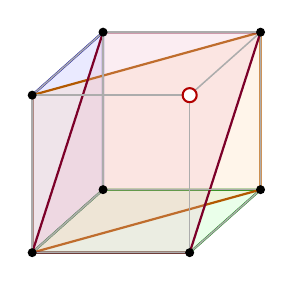
\begin{tikzpicture}[
    line cap=round,
    line join=round,
    edge/.style={draw=gray!65, line width=0.55pt},
    frontedge/.style={draw=black, line width=0.65pt},
    vertex/.style={circle, fill=black, inner sep=1.15pt},
    missing/.style={circle, draw=red!70!black, fill=white, line width=0.75pt, inner sep=1.8pt},
    faceA/.style={fill=blue!35,   draw=blue!60!black,   fill opacity=0.23, line width=0.8pt},
    faceB/.style={fill=green!35,  draw=green!50!black,  fill opacity=0.23, line width=0.8pt},
    faceC/.style={fill=orange!35, draw=orange!70!black, fill opacity=0.23, line width=0.8pt},
    faceD/.style={fill=purple!30, draw=purple!65!black, fill opacity=0.23, line width=0.8pt}
]

\begin{scope}[shift={(15.0,4.8)}]
  \coordinate (A) at (0,0);
  \coordinate (B) at (2,0);
  \coordinate (C) at (0,2);
  \coordinate (D) at (2,2);
  \coordinate (E) at (0.9,0.8);
  \coordinate (F) at (2.9,0.8);
  \coordinate (G) at (0.9,2.8);
  \coordinate (H) at (2.9,2.8);

  \filldraw[faceA] (A)--(C)--(G)--(E)--cycle;
  \filldraw[faceB] (A)--(B)--(F)--(E)--cycle;
  \filldraw[faceC] (A)--(C)--(H)--(F)--cycle;
  \filldraw[faceD] (A)--(B)--(H)--(G)--cycle;

  \draw[edge] (A)--(B)--(D)--(C)--cycle;
  \draw[edge] (E)--(F)--(H)--(G)--cycle;
  \draw[edge] (A)--(E);
  \draw[edge] (B)--(F);
  \draw[edge] (C)--(G);
  \draw[edge] (D)--(H);

  \node[vertex]  at (A) {};
  \node[vertex]  at (B) {};
  \node[vertex]  at (C) {};
  \node[missing] at (D) {};
  \node[vertex]  at (E) {};
  \node[vertex]  at (F) {};
  \node[vertex]  at (G) {};
  \node[vertex]  at (H) {};
\end{scope}
\end{tikzpicture}
\end{center}
Then one would like to set the lower face to be constant $x_0$,
the left face to be the element $a\in\pi_2(X,x_0)$ whose inverse we wish to construct,
and the diagonal $[x_1=x_2]$ to be also constant $x_0$.
But then there is the diagonal $[x_1=x_3]$ left,
whose second inert (= lower) face has to be equal to the 1-dimensional diagonal of $a$,
while having constant $x_0$ on the opposite (= upper) face and on the first inert (= lower) face.
But there is no guarantee for this 2-cube to exist in $X$.

The failure can be fixed if $X$ arises from a concrete cubeset
since then the points suffice to determine the face $[x_1=x_3]$ uniquely.
In particular, in the proof of Proposition~\ref{prop:concrete-structure-group-is-group} no flip is required (if one performs the same Definitions as before, beginning from Construction~\ref{cons:structure-monoid-concrete}).
\end{remark}

Let us close this section with the result that the structure groups of a concrete fibrant cubeset
can be equally computed over $\bbox$ or over $\bbGamma$.

\begin{proposition}
Let $X$ be a concrete fibrant cubeset and $x_0\in X$.
Then there is an isomorphism $\pi_n(X,x_0)\simeq\pi_n^{\bbGamma}(j^\ast X,x_0)$.
\end{proposition}

\begin{proof}
The $\bbGamma$-set $j^\ast(X/\sim_n)$ is $n$-step over $\bbGamma$:
since $X/\sim_n = \tau_n X$ is $n$-step over $\bbox$ by Proposition~\ref{prop:trunc_concfib},
it is $\Lambda_n$-local, and thus $j^\ast(X/\sim_n)$ is $\Lambda_{\bbGamma,n}$-local by concreteness
and Proposition~\ref{prop:nilfib-restricted-nilfib-concrete}.
Hence $\tau_n^{\bbGamma}(j^\ast(X/\sim_n),x_0)) = \pi_n^{\bbGamma}(j^\ast(X-/\sim_n),x_0)$
and from the explicit definition of structure monoid over $\bbGamma$
it is immediate that $\pi_n^{\bbGamma}(j^\ast(X/\sim_n),x_0) = \pi_n(X/\sim_n,x_0)$.

Thus, it suffices to show that
$\pi_n^{\bbGamma}(j^\ast(X/\sim_n),x_0)\simeq\pi_n^{\bbGamma}(j^\ast X,x_0)$.
By the universal property of $\tau_n^{\bbGamma}j^\ast X = X/\approx_n$,
see Proposition~\ref{prop:trunc-concfib-gamma}, there is a commutative diagram
\begin{center}
\begin{tikzcd}
	{j^\ast X} & {X/\approx_n} \\
	& {j^\ast(X/\sim_n)}
	\arrow["{\eta^{\bbGamma}}", from=1-1, to=1-2]
	\arrow["{j^\ast(\eta)}"', from=1-1, to=2-2]
	\arrow["f", dashed, from=1-2, to=2-2]
\end{tikzcd}.
\end{center}
We show that the monoid homomorphism
\begin{align*}
    f_\ast\colon\{c\in (X/\approx_n)(n) \mid c\rvert_{{\bbcor}^n_1}\equiv x_0 \}
    &\to\{c\in j^\ast(X/\sim_n)(n) \mid c\rvert_{{\bbcor}^n_1}\equiv x_0 \}, \\
    c&\mapsto f(c)
\end{align*}
is bijective.
For surjectivity take $c\in(X/\sim_n)(n)$ with $c\rvert_{{\bbcor}^n}\equiv x_0$.
Take $c'\in X(n)$ with $\eta(c') = c$.
Using universal replacement we can assume that $c'(0) = x_0$.
This then yields $d = \eta^{\bbGamma}(c') \in (X/\approx_n)(n)$ with $d\rvert_{{\bbcor}^n_1}\equiv x_0$
and $f(d) = c$.
For injectivity let $c,d\in\pi_n^{\bbGamma}(X/\approx_n,x_0)$ with $f(c) = f(d)$.
Take $c',d'\in (j^\ast X)(n) = X(n)$ with $\eta^{\bbGamma}(c') = c$, $\eta^{\bbGamma}(d') = d$,
in particular $c'(0) = x_0 = d'(0)$.
Moreover,
\[
    \eta(c') = f(\eta^{\bbGamma}(c')) = f(c) = f(d) = \eta(d').
\]
This means that for all $\omega\neq 0$ we have that $c'(\omega) \sim_n d'(\omega)$.
But this implies that $c = \eta^{\bbGamma}(c') = \eta^{\bbGamma}(d') = d$.
So $f_\ast$ is a monoid isomorphism.
\end{proof}

\begin{corollary}
If $X$ is a concrete fibrant cubeset, then $\pi_n^{\bbGamma}(j^\ast X,x_0)$ is grouplike for all $n\in\N$.
\end{corollary}
